\chapter{Mechanizmy mediacji wiedzy}
\label{cha:mechanizmyMediacjiWiedzy}

%---------------------------------------------------------------------------

\section{Obszary zastosowań}
\label{sec:obszaryZastosowan}

Z mechanizmami mediacji wiedzy spotykamy się na co dzień -- od prostych, analogowych form zebrania tzw. \textit{feedbacku} od użytkownika do bardziej zaawansowanych systemów cyfrowych.

Wiele instytucji publicznych (jak urzędy \cite{umkrakow}, szkoły, uczelnie \cite{wgigagh}) oraz prywatnych przedsiębiorstw gromadzi informacje od petentów czy klientów na przykład w formie dobrowolnych kwestionariuszy w~~celu podniesienia jakości świadczonych usług. W marketach popularność zyskują na przykład przyciski wformie emotikon, które klient może  nacisnąć przy wyjściu, przekazując czy jest zadowolony.

\begin{figure}[H]
	\centering
	\includegraphics[scale=0.8]{rozdzial2/Biedronka.jpg}
	\caption{Przykład prostego mechanizmu mediacji wiedzy w supermarketach sieci Biedronka. Użytkownik przekazuje informację o stanie afektywnym klikając w odpowiednią emotikonę.}
\end{figure}

	
Opinia osób jest szczególnie ważna w systemach tworzonych w sposób zorientowany na użytkownika (ang. \textit{user-centered design}). Na przykład w branży projektowania stron internetowych przy projektowaniu nowoczesnych, profesjonalnych rozwiązań, w fazie początkowych testów, a czasem również w~fazie regularnego funkcjonowania udostępnia się użytkownikowi kwestionariusz w celu poprawy jakości czy nawet buduje z grona użytkowników zespoły scrumowe odpowiedzialne, za przekazanie swoich odczuć związanych z designem \cite{uxdesign}.
	
Część systemów rekomendacji zaczęła już wykorzystywać mediację wiedzy. To rozwiązanie staje się coraz popularniejsze na przykład pośród platform zawodowo-biznesowych wykorzystywanych do poszukiwania pracy \cite{careerexplorer}.
	
Omawiane tu mechanizmy znajdują zastosowanie również w medycynie. Przykładem może być wspomniana już w poprzednim rozdziale aplikacja zaprojektowana w ramach pracy \cite{hung2016predicting} stanowiąca próbę walki z depresją.


%---------------------------------------------------------------------------

\section{Jawne metody mediacji wiedzy}
\label{sec:jawneMetodyMediacjiWiedzy}

Pierwszą z~kategorii metod mediacji wiedzy są metody jawne. Oznacza to, że w~proces mediacji zaangażowany jest sam użytkownik. To rozwiązanie ma swoje wady i zalety. Z pewnością największą zaletą jest skuteczność rozwiązania -- nikt nie wie więcej o stanie emocji niż sam użytkownik. Z kolei główną wadą jest fakt, że takie badanie może okazać się uciążliwe i irytujące, a na dłuższą metę zbytnio ingerujące w~życie człowieka, czy wręcz niemożliwe.

Przykładem jawnej metody może być praca \cite{EmiliaPieczonka}. W badaniach, jakie przeprowadziła, ''grupa użytkowników korzystajaca z~telefonu Android i aplikacji mobilnej, używała podczas codziennych czynności urządzenia sensorycznego na swoim nadgarstku i odpowiadała na pytania dotyczące ich samopoczucia''.

Warto również zwrócić uwagę na pracę \cite{ArkadiuszLis}. Zostało w~niej wybrane w~oparciu o literaturę naukową kilka najbardziej obiecujących sposobów mediacji wiedzy. Następnie zaimplementowano zestaw widgetów, z~pomocą których użytkownik ''powinien być w~stanie subiektywnie określić stan emocjonalny (...), a następnie przekazać tą informację do systemu''.

W pracy opisanej w~artykule \cite{hung2016predicting} naukowcy we współpracy z~psychiatrą stworzyli system, z~którego pomocą badany z~wykorzystaniem kolorowego suwaka może określić poziom swojego niepokoju czy gniewu. Badacze skupili się przede wszystkim nie na sensorach, ale na wzorcach korzystania z~telefonu udostępniach przez system operacyjnych takich jak wykonywanie połączeń, pisanie SMSów czy lokalizacja.

Mediacja nie musi odbywać się z~wykorzystaniem ekranu. Na rynku pojawiają się rozwiązania, w~których system głosowy taki jak Alexa, Asystent Google, Cortana czy Siri podczas rozmowy sam wypytuje użytkownika o nastrój.


%---------------------------------------------------------------------------

\section{Niejawne metody mediacji wiedzy}
\label{sec:niejawneMetodyMediacjiWiedzy}

Drugą kategorią metod mediacji wiedzy są metody niejawne. De facto sprowdza się to do braku bezpośredniego uczestnictwa człowieka w~przekazywaniu wiedzy. Oczywiście człowiek jest zaangażowany w~proces na przykład poprzez wykonywanie różnych czynności, ale nie zostanie nigdy zapytany wprost. Podobnie jak pierwsza kategoria, ta druga również ma swoje wady i zalety. Do zalet można zaliczyć wygodę -- korzystanie z~tych metod jest nieinwazyjne, nie ingeruje w~codzienną egzystencję. Minusem jest oczywiście mniejsza skuteczność.

Przykładem takiej mediacji może być praca \cite{zhang2011feature}, w~której naukowcy podejmują próby rozpoznania aktywności człowieka wykorzystując czujniki multimodalne. Do przetworzenia danych wykorzystywane są algorytmy wyboru cech.

Podobną metodą wykorzystali naukowcy w~pracy \cite{dai2010mobile} wykorzystując stworzony przez siebie model matematyczny w~celu określenia czy kierowca samochodu jest trzeźwy czy pijany.


%---------------------------------------------------------------------------

\section{Pozyskiwanie wiedzy o stanie emocjonalnym w~systemach \textit{affective computing}}
\label{sec:pozyskiwanieWiedzyOStanieEmocjonalnymWSystemachAffectiveComputing}

\textit{Affective computing} jest paradygmatem zaproponowanym przez Rosalind Picard z~Laboratorium Mediów MIT w~1997 roku\cite{picard1997affective}.

Wykorzystuje on rezultaty inżynierii biomedycznej, psychologii i sztucznej inteligencji. Celem jest pozwolenie systemom komputerowym wykrywać, wykorzystywać, a nawet wyrażać emocje\cite{nalepa2017affective}.

Przykładem pozyskiwania wiedzy może być gra wideo \textit{Bridge Scroll-runner} stworzona w~ramach pracy \cite{nalepa2017affective}. Naukowcy rozszerzyli możliwości gry wykorzystując czujniki tętna, temperatury skóry oraz reakcji galwanicznej skóry.

Rosaling Picard w~swojej pionierskiej pracy \cite{picard1997affective} jako przykład podaje komputerowy system uczący gry na pianinie. Taki system mógłby być znacznie skuteczniejszy od klasycznego systemu dysponując możliwością wyczuwania zainteresowania, przyjemności i smutku.

Wraz z rozwojem technologii metody pozyskiwania wiedzy o stanie emocjonalnym stają się coraz bardziej zaawansowane. Realizacja kolejnych technik jest dla twórców swego rodzaju wyzwaniem, ale stanowi okazję do przeprowadzenia coraz dokładniejszej analizy ludzkich emocji. Poniżej przedstawiono przegląd znanych metod pozyskiwanie wiedzy o stanie emocjonalnym w~systemach \textit{affective computing}:

\begin{itemize}	
	\item Najbardziej podstawowymi metodami są techniki analogowe. Kwestionariusz może być przeprowadzony w sposób całkowicie niewspomagany cyfrowo. Sposób polega na tym, że osobie badanej zostaje przedstawiony zestaw pytań. Mamy tutaj szeroki zakres możliwości. Pytania mogą być wypełniane przez uczestnika badania lub zadawane przez ankietera -- w tym drugim przypadku ankieter może próbować również skonstruować kolejne, bardziej dokładne pytania. Kwestionariusz może być wypełniony przez osobę jednorazowo lub wypełniany w sposób regularny -- te bardziej systematyczne z reguły dają lepsze rezutaty. Same pytania mogą dotyczyć stanu obecnego, mogą też dotyczyć stanów z przeszłości. W bardziej zaawansowanych wersjach dodatkowe pytania mogą pomóc zrozumieć nie tylko stan, ale także czynniki czy okoliczności, które przyczyniły się do jego zmiany. Jedną z zalet kwestionariuszy jest fakt, że można zdobyć info bez konieczności poświęcenia czasu i zasobów na projektowanie i implementacje bardziej zaawansowanego techologicznie rozwiązania. Przeprowadzony w sposób dokładny i regularny może dać zadowalające wyniki. Trzeba też pamiętać, że przez lata była to jedyna dość skuteczna metoda. Z kolei zedycowaną wadą jest fakt, że metoda ta może być bardzo obciążająca zarówno dla osoby badanej jak i badającej. Im bardziej szczegółowe badanie, z tym większą uciążliwością się to wiąże. Samo podejście może się okazać czasochłonne, a wyniki trudne do opracowania.
	
	\item Inną, nieco bardziej zaawansowaną metodą jest wykonywanie połączeń telefonicznych tak jak w~badaniu \cite{courvoisier2010psychometric}. W porównaniu do techniki analogowej jest to bardziej wymagające przede wszystkim logistycznie, a główną wadą może być znaczne obciążenie zarówno strony badającej jak i badanej.
	
	\item Odmienne podejście prezentują automatyczne techniki gromadzenia informacji o stanie emocjonalnym użytkownika. Mowa tu o systemach, które regularnie co jakiś czas przedstawiają osobie badanej pytanie i zapisują odpowiedź. W tym przypadku wyzwaniem jest wybór platformy i przede wszystkim stworzenie sytemu, ale zmiana podejścia daje duże zyski w postaci automatyzacji całego procesu.
	
	\item Bardziej zaawansowanym sposobem jest wybór zakresów godzinowych (czyli pór dnia) poprzez eksperta domenowego i tym samym ograniczenie odpytywania uczestnika badania tylko do określonych przedziałów. Technika mediacji o losowej porze, ale tylko wewnątrz ustalonego wcześniej zakresu została zastosowana m.in. w pracy \cite{bailon2019smartphone}. W tym przypadku zaletą jest nieznaczne obciążenie techniczne w stosunku do poprzedniej metody. Zmiana w postaci zawężenia okresów odpytywania niewielkim kosztem sprawia, że system jest bardziej przyjazny dla użytkownika.
	
	\item Ostatnią z przytoczonych tutaj metod jest odpytywanie użytkownika w czasie rzeczywistym w~oparciu o wnioskowanie na podstawie danych z otoczenia. System, który jest świadomy ,,kontekstu'' (ang. \textit{context-aware system}) jest w stanie zminimalizować uciążliwość dla użytkownika odpytując na przykład tylko w momentach, kiedy nie jest pewny stanu emocjonalnego (bo na przykład może go zbadać również w sposób niejawny), albo zaobserwował znaczącą zmianę jednego z czynników otoczenia. Właśnie taka zaawansowana aplikacja stworzona zostanie w ramach niniejszej pracy.
\end{itemize}

W pracy zastosowano zarówno metody jawne jak i niejawne. W celu pozyskania wiedzy o stanie emocjonalnym zdecydowano się na syntezę odpowiedzi użytkownika i działania automatycznego systemu. Odpowiedzi użytkownika mogą być realizowane wprost poprzez aktywność z~listą emocji (jak na powyższym diagramie) i emotikon do wyboru lub (bardziej psychologicznie) z~wykorzystaniem palety kolorów. Automatyczny system wykorzystuje zewnętrzne API, które zwraca wartości wykrytych emocji na podstawie fotografii, która została wcześniej wykonana. W przyszłości możliwe jest rozszerzenie aplikacji o system uczący się rozpoznawać emocje z~sensorów AWARE porównując duże ilości danych niezrozumiałych z~sensorów z~danymi otrzymanymi z~wykorzystaniem jawnych i niejawnych metod mediacji wiedzy.

\begin{figure}[H]
	\centering
	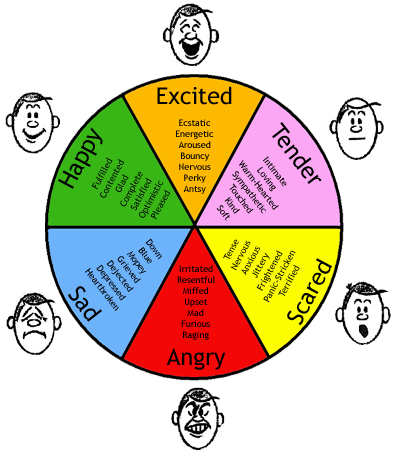
\includegraphics[scale=1]{rozdzial2/ModelEkmana.png}
	\caption{Koło podstawowych emocji (szczęście, podekscytowanie, rozczulenie, strach, gniew i smutek) i ich mimicznych ekspresji.}
\end{figure}

